\cleardoublepage
\chapter{Software}
% To do: 
% Color Scheme
% Red - Not started
% Yellow - In progress
% Blue - Done, under approval
% Green - Done and approved
\todo[inline,color=red!40]{*Chapter Introduction}
\todo[inline,color=blue!40]{*1 - Microphone}
\todo[inline,color=blue!40]{ a) WOMic}
\todo[inline,color=red!40]{*2 - Accelerometer and Piezoelectric}
\todo[inline,color=red!40]{ a) Microcontroller}
\todo[inline,color=red!40]{ c) FFT implementation}
\todo[inline,color=red!40]{*3 - MatLab}
%%%%%%%%%%%%%%%%%%%%%%%%%%%%%%%%%% Writing %%%%%%%%%%%%%%%%%%%%%%%%%%%%%%%%%%%
\section{Microphone}
As the first measurements will be taken recurring to a microphone, it requires a different approach to the type of interaction when compared to the future application, were will be use a different sensor for the vibration. To obtain access and record the information from the microphone and for this case in specific, since is being used the microphone from a phone, will require different pieces of software to use in the phone side and the PC, to allow the access to the second to the microphone of the first. Also, on the PC side is necessary to record the information from the microphone and store it as desire.\\
The two components for this purpose will be the use of the WOMic software as the bridge between the phone and the computer, and MATLAB to record the information from the microphone. The second software can also be used to latter process the recorded data, helping the understand of the obtained information. 
\subsection*{WOMic}
The use of the application and the microphone of the phone is simple, although the installation and the configuration requires some time. For that, is required to install the software \textit{WOMic} in both devices, this allow to use the microphone of the phone in real-time. In the phone the software is available for Android and IOS and is responsible to transmit what is captured from the microphone, in the computer the client application and a virtual device must be installed to use the microphone in the PC to perform any type of tasks, this connection can be made over USB, Bluetooth, Wi-Fi and Wi-Fi Direct.\\ 
In order to save what is captured from the microphone, the software is split in three main block with different purposes, the \textit{WOMic App} runs in the phone, samples the input of the microphone and transmit it to the computer, the \textit{WOMic Client}, runs in the PC, connect to the app in the phone, and receive the data from the microphone, which is transmitted to the \textit{WOMic Virtual Device} on which a real microphone device is simulated and provides the audio to any application or program in the PC, as illustrated in figure \ref{fig:diagramWOMIC}.\\
\begin{figure}[!htb]
    \centering
    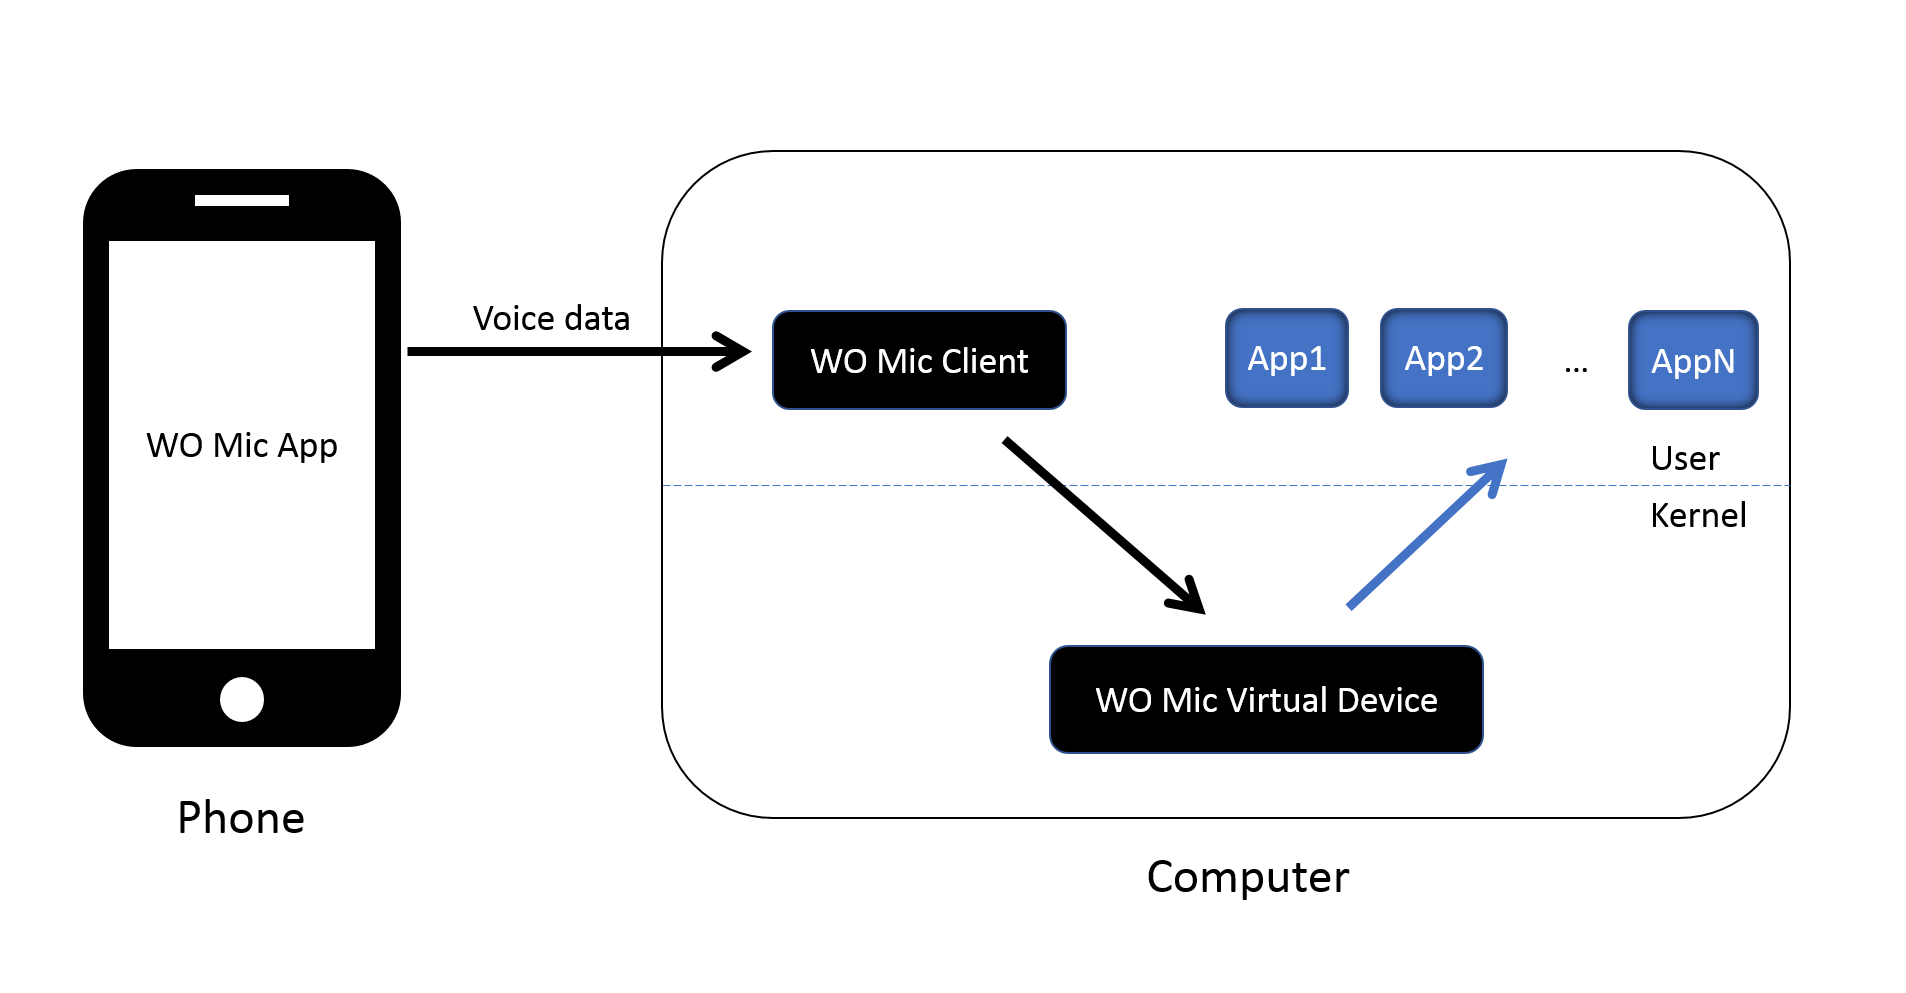
\includegraphics[width=0.65\textwidth]{Chapters/5CHP/Images/WOMICDiag.png}
    \caption{Flow of data in the components of the software}{\cite{WOMicFREE}}
    \label{fig:diagramWOMIC}
\end{figure}
In addition to this, is also necessary to install the drivers of the phone in use, if the connection is made over USB. To allow the access of the microphone in the PC, the transport mode must be selected on the phone application, USB in this case, in the app settings and after that start the application. In the PC the client software must be initialized and connected to the phone in the following order \textit{\>Connection\>Connect...} a new window will open, on which the USB must be selected as transport type and finalizing by pressing \textit{Connect}. With this, the microphone of the phone is available for use in the PC\cite{WOMicFREE}.
\section{Microcontroller}
%Introduction
%What is the purpose of each used element, Timer, UART, ADC, PINOUT for solenoid with timer
%What are the config of each
% Mainly from the ADC and how it works without having to use an additional timer
%
\subsection*{Timers}
\subsection*{ADC}
The LaunchPad in use offers ADC with a 10-bit, from the availabed pins, analog input 2 is selected. This input should be configured with the desire setting, to start is mandatory to disable the digital port of the pin to eliminate the flow of parasitic current flow, with the PySELx bits, by setting this bits HIGH it automatically enables the analog function of the port, although is still necessary to select the channel to conversion. The ADC will function in the sample and hold mode, using the timer from the ADC as the source of the sampling signal, the sample and hold period can be changed by software, to define the amount of clock cycles between each sample. 
\subsection*{UART}
\section{MatLab}
\section{FFT implementation}

%%%%%%%%%%%%%%%%%%%%%%%%%%%%%%%%%%%%%%%%%%%%%%%%%%%%%%%%%%%%%%%%%%%%%%%%%%%%%%

\section{??}
% \begin{figure}[!htb]
%     \centering 
%         \begin{subfigure}[c]{\textwidth}
%             \centering
%             \input{Sections/3Transforms/Images/DFTSymmetry.tex}
%             \caption{}
%             \label{subfig:dft}
%         \end{subfigure}
%         \begin{subfigure}[c]{0.45\textwidth}
%             \centering
%             \input{Sections/3Transforms/Images/DCT1Symmetry.tex}
%             \caption{}
%             \label{subfig:dct1}
%         \end{subfigure}
%         \begin{subfigure}[c]{0.45\textwidth}
%             \centering
%             \input{Sections/3Transforms/Images/DCT2Symmetry.tex}
%             \caption{}
%             \label{subfig:dct2}
%         \end{subfigure}
%         \begin{subfigure}[c]{0.45\textwidth}
%             \centering
%             \input{Sections/3Transforms/Images/DCT3Symmetry.tex}
%             \caption{}
%             \label{subfig:dct3}
%         \end{subfigure}
%         \begin{subfigure}[c]{0.45\textwidth}
%             \centering
%             \input{Sections/3Transforms/Images/DCT4Symmetry.tex}
%             \caption{}
%             \label{subfig:dct4}
%         \end{subfigure}
%         \caption{Sequences generated in the first step of Table \ref{tab:DFTDCT}for the DFT and different DCTs. Filled dots correspond to the original sequence ((a) - \emph{DFT}; (b)) - \emph{DCT-I}; (c)) - \emph{DCT-II}; (d)) - \emph{DCT-III}; (e)) - \emph{DCT-IV}).}
%     \label{fig:2NSeq}
% \end{figure}
% \begin{lstlisting}
%     ./aomenc <INPUT-FILE> -h <HEIGHT> -w <WIDTH> -o <OUTPUT-FILE> --limit=10 -p 1 --cpu-used=8 --i420 --q-hist=64 --end-usage=q --cq-level=<CQ-LEVEL>
% \end{lstlisting}
%\addcontentsline{toc}{section}{References}
